% !TEX TS-program = LilyPond-Book2011

%%%%%PREAMBULE%%%%%

\documentclass[a4paper,11pt,bibliography=totoc,numbers=noenddot,listof=flat,DIV=11,BCOR=0mm]{scrreprt}%{scrbook}scrreprt
%\usepackage[top=3 cm, bottom=3 cm, left=2.5 cm, right=2.5 cm]{geometry}

\usepackage{flupstyleutfbook}
\usepackage[parfill]{parskip}
  

\usepackage{url}
\usepackage{ae}
\usepackage{microtype}
\usepackage{tabularx}
\usepackage{array}


\usepackage[automark]{scrpage2}
\pagestyle{scrheadings}
\clearscrheadfoot
\automark[section]{chapter}


\usepackage[bitstream-charter]{mathdesign}

\usepackage[hyperfootnotes=false,colorlinks=false,pdftex]{hyperref}
\hypersetup{ pdfinfo={
Title={Titre},
Subject={Sujet}, 
Author={Philippe Massart}, % ...
}
}

\usepackage{breakurl}

%\usepackage{makeidx}
%\makeindex
\KOMAoptions {listof=totoc}
\KOMAoptions  {index=totoc}
\renewcommand*{\partpagestyle}{empty}

\usepackage{tikz}
\usetikzlibrary{arrows}
\usetikzlibrary{trees} % LATEX and plain TEX
\usepackage{pgfplots}
\usepackage{verbatim}


\usepackage{caption}
\addto\captionsfrench{\def\figurename{{\bf Fig.}}} % Pour que les titres ne soient plus en smallcaps, soient en gras et soient Fig. au lieu de Figure.

\DeclareGraphicsExtensions{.pdf, .jpg, .tif, .gif}
%\AddThinSpaceBeforeFootnotes



%%%%%%Aligner les footnotes sur le début du texte et non de la marge%%%%%
\makeatletter
\long\def\@makefntextFB#1{%
	\ifx\thefootnote\ftnISsymbol
		\@makefntextORI{#1}%
	\else
		\rule\z@\footnotesep
		\setbox\@tempboxa\hbox{\@thefnmark}%
			\ifdim\wd\@tempboxa>\z@
				\kern2em\llap{\@thefnmark.\kern0.5em}%
			\fi
		\hangindent2em\hangafter\@ne#1
	\fi}
\makeatother
%%%%%%%%%%%%%%%%%%%%%%%%%%%%%%%%%%%%%%%%%




\newcommand{\betweenLilyPondSystem}[1]{\vspace{5mm}\linebreak}

\addto\captionsfrench{%
  \renewcommand{\chaptername}%
    {Préparation}%
}

\usepackage[multiple,stable]{footmisc}

%%%%FIN PREAMBULE%%%%%


\begin{document}
\thispagestyle{empty}
\begin{center}
\begin{LARGE} \textbf{\textsc{Fiches de préparations}\\ \vspace{1cm}} 
\end{LARGE}  \vspace{2cm}
 {\Large \textsc{Philippe Massart}}
 \vspace{16.5cm}
\\ \textsc{Didactique générale -- Créativité\\ Cours de Sarah Goldfarb\\ Janvier 2012}
\end{center}


\pagenumbering{arabic}
\renewcommand{\headfont}{\normalfont\rmfamily\scshape}
%\setfootsepline[14,91cm]{0.4pt}
%\setfootbotline[14,91cm]{0.4pt}
\setheadsepline[15.273cm]{0.4pt}
\ihead{Didactique -- Créativité}
\ohead{\chaptername{} \headmark}
\cfoot[-- \pagemark{} --]{-- \pagemark{} --}

\tableofcontents
\ohead{\headmark}


\vspace{1cm}
\begin{doublespace}
La réalisation de ce travail a été rendue possible par les outils informatiques suivants:
\begin{itemize}
\item \LaTeX
\item GNU LilyPond
\item Apple Pages
\end{itemize}
\end{doublespace}


%%%%%%%%%%%
%JEU DE COM 1%
%%%%%%%%%%%
\chapter[Jeu de communication: Prénoms]{Prénoms}
\chaptermark{Prénoms}
\ohead{\chaptername{} \headmark}
%pulsations -> nom -> nom + celui d'un autre -> attendre x pulsations avant la suite (en fct du travail prévu au cours) ou sur un rythme à travailler par après

%{\large \textbf{Sous-titre}}:
% ???

%\subsection*{Catégorie}
{\large \textbf{Catégorie}}:
jeu de communication

\section*{Cadre et public}
\begin{itemize}
\item [\textbullet]\textbf{Type d'atelier} : cours d'instrument ou d'ensemble instrumental

\item [\textbullet]\textbf{Public} : élèves de tous âges ne se connaissant peu ou pas (en début d'année pour l'ensemble, avant une audition de classe pour les cours d'instruments)

\item [\textbullet]\textbf{Gestion du temps} : 5 à 10 minutes, selon le nombre d'élèves

\item [\textbullet]\textbf{Matériel} : local avec un espace libre pour que les élèves puissent se placer en cercle
\end{itemize}

\section*{Objectifs}
\begin{itemize}
\item connaître le prénom de chacun
\item écoute d'une pulsation proposée par un des participants
\item intégration de la pulsation dans une métrique proposée
\end{itemize}

\subsection*{Difficultés possibles}

\section*{Déroulement par étapes}
\begin{itemize}
\item une métrique est choisie en fonction du morceau à travailler pendant la suite du cours (\metric{3}{4}, \metric{4}{4}~etc.) 
\item un des participants propose une pulsation sur cette métrique
\item tout le monde frappe la pulsation proposée dans les mains
\item dans le sens des aiguilles d'une montre, chacun dit son nom sur le premier temps, en laissant passer une mesure entre chacun
\item après un tour, celui qui dit son nom dit également le nom d'un autre participant qui fera pareil (une mesure pour son nom, une mesure pour celui du suivant)
\item on arrête lorsque le nom de chacun a dit son nom 2 fois
\end{itemize}


%%%%%%%%%%%
%JEU DE COM 2%
%%%%%%%%%%%
\chapter[Jeu de communication: Prénom et instrument]{Prénom et instrument}
\chaptermark{Prénom et instrument}

%{\large \textbf{Sous-titre}}:
% ???

%\subsection*{Catégorie}
{\large \textbf{Catégorie}}:
jeu de communication

\section*{Cadre et public}
\begin{itemize}
\item [\textbullet]\textbf{Type d'atelier} : cours d'ensemble instrumental ou de formation musicale

\item [\textbullet]\textbf{Public} : tous en ensemble instrumental; en formation musicale, les élèves déjà inscrits en formation instrumentale

\item [\textbullet]\textbf{Gestion du temps} : 5 à 10 minutes selon le nombre d'élèves

\item [\textbullet]\textbf{Matériel} : local avec un espace libre pour que les élèves puissent se placer en cercle
\end{itemize}

\section*{Objectifs}
\begin{itemize}
\item connaître le prénom et l'instrument de chacun
\item écoute d'une pulsation proposée par un des participants
\item intégration de la pulsation dans une métrique proposée
\end{itemize}

\subsection*{Difficultés possibles}
Pour les instruments moins connus (alto, certaines percussions, par exemple), on peut dans un premier temps remplacer les instruments par les familles d'instruments

\section*{Déroulement par étapes}
\begin{itemize}
\item une métrique est choisie en fonction du morceau à travailler pendant la suite du cours (\metric{3}{4}, \metric{4}{4}~etc.) 
\item un des participants propose une pulsation sur cette métrique
\item tout le monde frappe la pulsation proposée dans les mains
\item dans le sens des aiguilles d'une montre, chacun dit son nom sur le premier temps, en laissant passer une mesure entre chacun
\item après un tour, chacun remplace son nom par son instrument; sur la deuxième mesure, on désigne le participant suivant (par son prénom)
\item on arrête lorsque l'instrument de chacun a été dit 2 fois
\end{itemize}

%%%%%%%%%%%
%JEU ECHAUFF 1  %
%%%%%%%%%%%
\chapter[Jeu d'échauffement: Explosion de doigts]{Explosion de doigts}
\chaptermark{Explosion de doigts}

%{\large \textbf{Sous-titre}}:
% ???

%\subsection*{Catégorie}
{\large \textbf{Catégorie}}:
échauffement

\section*{Cadre et public}
\begin{itemize}
\item [\textbullet]\textbf{Type d'atelier} : cours de piano

\item [\textbullet]\textbf{Public} : 2 à 3 élèves, selon le nombre d'élève présents et la place disponible

\item [\textbullet]\textbf{Gestion du temps} : 5 minutes en début de cours

\item [\textbullet]\textbf{Matériel} : aucun
\end{itemize}

\section*{Objectifs}
\begin{itemize}
\item échauffement des mains
\item installation d'une pulsation ressentie physiquement
\end{itemize}

%\subsection*{Difficultés possibles}

\section*{Déroulement par étapes}
\begin{itemize}
\item marche sur place gauche-droite
\item fermer les poings
\item en même temps que le pas à gauche, ouvrir d'un coup la main, puis la refermer sur le pas à droite
\item répéter 5 fois, s'interrompre pendant 5 séquences de pas, puis refaire 5 fois
\end{itemize}


%%%%%%%%%%%
%JEU ECHAUFF 2  %
%%%%%%%%%%%
\chapter[Jeu d'échauffement: Tête, épaules et \ldots{}]{Tête, épaules et \ldots{}}
\chaptermark{Tête, épaules et \ldots{}}

%{\large \textbf{Sous-titre}}:
% ???

%\subsection*{Catégorie}
{\large \textbf{Catégorie}}:
échauffement

\section*{Cadre et public}
\begin{itemize}
\item [\textbullet]\textbf{Type d'atelier} : cours de piano

\item [\textbullet]\textbf{Public} : 2 à 3 élèves, selon le nombre d'élève présents et la place disponible

\item [\textbullet]\textbf{Gestion du temps} : 5 minutes en début de cours

\item [\textbullet]\textbf{Matériel} : aucun
\end{itemize}

\section*{Objectifs}
\begin{itemize}
\item détente du cou et des épaules, lieux de tensions fréquentes chez les pianistes
\end{itemize}

\subsection*{Difficultés possibles}
Pour les élèves ayant des soucis d'équilibre (les adultes plus âgés, par exemple), la détente du cou peut poser problème; il y aura alors lieu de faire cette partie de l'exercice assis

\section*{Déroulement par étapes}
\begin{itemize}
\item ancrage des pieds au sol
\item tourner lentement le cou dans le sens des aiguilles d'une montre, puis dans l'autre sens
\item lever un bras (tous dans le même sens et du même côté pour éviter les collisions) et décrire un cercle vers l'arrière; faire de même d'arrière en avant puis changer de bras
\end{itemize}



%%%%%%%%%%
%JUNGLE NOTES%
%%%%%%%%%%
\chapter[Jeu musical: Jungle notes]{Jungle notes}
\chaptermark{Jungle notes}


%\subsection*{Sous-titre}
{\large \textbf{Sous-titre}}:
 jeu musical sur le mode du jeu \emph{Jungle Speed}

%\subsection*{Catégorie}
{\large \textbf{Catégorie}}:
jeu musical

\section*{Cadre et public}
\begin{itemize}
\item [\textbullet]\textbf{Type d'atelier} : cours de piano

\item [\textbullet]\textbf{Public} : 3 élèves débutant le cours de piano après 9 mois à 1 an de formation musicale en cycle de formation (selon la longueur de la liste d'attente en piano); les élèves auront donc en général 7 à 8 ans.

\item [\textbullet]\textbf{Gestion du temps} : 5 à 10 minutes au début de 2\ieme{} cours, reproductible par la suite.

\item [\textbullet]\textbf{Matériel} : jeu de cartes comprenant une note par carte, avec portée et clé (sol ou fa). Selon que les élèves ont ou non des notions de clé de fa, les cartes \emph{clé de fa} seront utilisées (toutes ou certaines, selon le répertoire abordé) ou laissées de côté.
\end{itemize}

\begin{figure}[ht!]
\centerline
   {\fbox{\includegraphics{Cartes/carte_note.pdf}}}
\end{figure}


%\subsection*{Horaire et gestion du temps}

%\subsection*{Répertoire éventuel}



%\subsection*{Besoins}


\section*{Objectifs}
\begin{itemize}
\item exercice de lecture rapide
\item localisation des notes sur le clavier
\end{itemize}

\subsection*{Difficultés possibles}
En cas de difficulté récurrente de lecture chez un élève, il y a lieu de s'entretenir avec son professeur de formation musicale afin d'élaborer ensemble une stratégie pour remédier à ce problème

\section*{Déroulement par étapes}
(Echauffement, apprentissage, créativité)
\begin{itemize}
\item chaque élève s'assied au piano et pose ses mains sur le clavier de façon à couvrir l'entièreté d'une gamme de do majeur (p. ex. do ré mi fa à gauche, sol la si do à droite)
\item un autre élève ou le professeur leur montre une carte; dès qu'ils la voient, les élèves jouent la note. Le plus rapide gagne 1 point; une bonne note en donne 1 aussi. Le premier à 5 points a gagné.
\end{itemize}


%\subsection*{Feed-back possible}
%
%(Ce que vous pourriez dire aux participants)

\section*{Prolongements éventuels}
\begin{itemize}
\item [\textbullet] Réalisation pour les élèves d'un ensemble de cartes pour qu'ils puissent jouer chez eux, avec des amis.
\item [\textbullet] Utilisation des mêmes cartes avec d'autres règles: bataille (en déterminant si les graves ou les aigües sont les plus fortes), jeu de paires (en enlevant une carte) etc.

\end{itemize}


%%%%%%%%%%%
%KYUDO  %
%%%%%%%%%%%
\chapter[Jeu musical: Ky\={u}d\={o}]{Ky\={u}d\={o}}
\chaptermark{Ky\={u}d\={o}}

{\large \textbf{Sous-titre}}:
 jeu musical de repérage du clavier

%\subsection*{Catégorie}
{\large \textbf{Catégorie}}:
jeu musical

\section*{Cadre et public}
\begin{itemize}
\item [\textbullet]\textbf{Type d'atelier} : cours de piano

\item [\textbullet]\textbf{Public} : 2 à 3 élèves ayant au moins une année de pratique à l'instrument et ayant abordé des pièces où les mains changent de position en cours de partition

\item [\textbullet]\textbf{Gestion du temps} : 5 à 10 minutes au début de cours, reproductible fréquemment si besoin

\item [\textbullet]\textbf{Matériel} : 
\begin{itemize} 
\item piano et 2 à 3 chaises selon le nombre d'élèves.
\item éventuellement une partition sur le pupitre, pour attirer le regard des élèves.
\end{itemize}


%\subsection*{Horaire et gestion du temps}
 
%\subsection*{Répertoire éventuel}



%\subsection*{Besoins}


\section*{Objectifs}
\begin{itemize}
\item localisation des mains sur le clavier
\item utilisation de la vision périphérique
\item concordance entre le ressenti visuel et la localisation réelle de la main
\end{itemize}

\subsection*{Difficultés possibles}
Le pupitre d'un piano droit ou électrique est placé plus bas que sur un piano à queue; l'exercice sera donc plus difficile sur ce dernier

\section*{Déroulement par étapes}
\begin{itemize}
\item les élèves posent les mains au clavier mais regardent le pupitre
\item un des élèves donne le nom d'une note; à ce moment (et le plus rapidement possible), les autres jouent cette note, toujours sans regarder le clavier
\item celui qui a donné le départ vérifie la justesse de la note et la rapidité. Le plus rapide obtient un point, une note juste également
\item c'est au tour d'un autre élève de donner la note à jouer
\item le jeu se termine quand 5 notes auront été jouées. On fait le total de point
\end{itemize}


%\subsection*{Feed-back possible}
%
%(Ce que vous pourriez dire aux participants)
%
%\section*{Prolongements éventuels}
%\begin{itemize}
%\item [\textbullet] test

\end{itemize}

%%%%%%%%%%%
%SOUNDPAINTING%
%%%%%%%%%%%
\chapter[Soundpainting: L'entrelac des signes]{L'entrelac des signes}
\chaptermark{L'entrelac des signes}

{\large \textbf{Catégorie}}: soundpainting\footnote{Les signes choisis pour représenter les différentes instructions de jeu ont été développés sur base de deux références : 
\begin{itemize}
\item interview de Walter Thompson à propos de ses choix de notation et de l’utilisation de Finale: %\footnote{
\href{http://www.newmusicbox.org/articles/How-does-using-music-notation-software-affect-your-music-Walter-Thompson/}{http://www.newmusicbox.org/articles/How-does-using-music-notation-software-affect-your-music-Walter-Thompson/}
%}
\item dossier pédagogique disponible sur {\href{http://www.soundpainting.be/docs/Dossier{ }SP{ }Ecoles{ }papier.pdf}{http://www.soundpainting.be/docs/Dossier{ }SP{ }Ecoles{ }papier.pdf}}
\end{itemize}


Les autres signes ont été choisis en fonction de leur ressemblance avec des gestes utilisés en soundpainting ou d'après les travaux de Kurt Stone (\emph{Music Notation in the Twentieth : A Practical Guidebook}, New York: Norton, 1980)}

\section*{Cadre et public}
\begin{itemize}
\item [\textbullet]\textbf{Type d'atelier} : ensemble instrumental et formation musicale (si les élèves suivent déjà un cours d'instrument par ailleurs)

\item [\textbullet]\textbf{Public} : tous, pourvu qu'ils aient déjà quelques notions de la syntaxe de soundpainting

\item [\textbullet]\textbf{Gestion du temps} : à répartir sur plusieurs cours

\item [\textbullet]\textbf{Matériel} : local avec au moins un piano; l'instrument de chaque élève

\end{itemize}

\section*{Objectifs}
\begin{itemize}
\item développer le regard hors partition
\item intégrer des compétences acquises dans un cadre non figé
\end{itemize}

%\subsection*{Difficultés possibles}

\section*{Déroulement par étapes}
(Echauffement, apprentissage, créativité)
\begin{itemize}
\item contrôle de la connaissance des différents éléments de syntaxe de soundpainting
\item exécution de la "partition"
\end{itemize}





%\begin{figure}[HT!]
%\centerline{
%\includegraphics[
%%scale=0.60,
%width=17cm,angle=90]{Soundpainting.pdf}
   %}
%\end{figure}
\includepdf[pages={1},angle=90,pagecommand={}, scale=0.80]{Soundpainting.pdf}
\includepdf[pages={2},angle=90,pagecommand={}, scale=0.80]{Soundpainting.pdf}
\includepdf[pages={3},angle=90,pagecommand={}, scale=0.80]{Soundpainting.pdf}

%%%%%%%%%%%%%
%PARTITION OUVERTE%
%%%%%%%%%%%%%
\chapter[Partition ouverte: Atomium]{Atomium}
\chaptermark{Atomium}
{\large \textbf{Catégorie}}:
partition ouverte

\section*{Cadre et public}
\begin{itemize}
\item [\textbullet]\textbf{Type d'atelier} : élèves d'ensemble instrumental ou musique de chambre ayant terminé le cycle de formation musicale, éventuellement en collaboration avec les classes d'instruments. Possibilité de collaboration avec les classes d'arts de la parole.

\item [\textbullet]\textbf{Public} : élèves adultes

\item [\textbullet]\textbf{Gestion du temps} : à répartir sur plusieurs cours

\item [\textbullet]\textbf{Matériel} : un grand local, un ou plusieurs claviers, l'instrument de chaque participant
\end{itemize}

\section*{Objectifs}
\begin{itemize}
\item décryptage d'une notation particulière
\item respect d'instructions précises
\item mise en perspective avec l'actualité
\end{itemize}

%\subsection*{Difficultés possibles}

\section*{Déroulement par étapes}
\begin{itemize}
\item découverte de la partition
\item propositions d'interprétation des signes, avant le recours aux instructions
\item découverte des instructions et comparaison avec les propositions de l'étape précédente
\item travail collectif des différents fragments
\item choix collégial d'un responsable de la pulsation
\item choix (individuel et éventuellement non exprimé) du fragment de chacun
\end{itemize}


\newpage	
\section*{Instructions}
L'effectif instrumental est indéterminé. Les instruments à sons à hauteur indéterminée exécutent le rythme en tenant compte, dans la mesure du possible, des différences de hauteurs indiquées (toms de hauteurs différentes, par exemple). Avant le début de l'exécution, un \emph{informateur} est choisi, qui donnera le signal de départ.

\subsubsection*{Partie I: \og Information \fg{}}
Les participants (seuls ou groupés) jouent une cellule rythmique de leur choix parmi les propositions de la Partie I, sur une des notes du mode acoustique\footnote{Appelé également gamme Bartók, mode lydien dominant ou Vaschaspati en musique hindoue.}\footnote{Puisqu'\emph{in fine}, les groupes devront finir par s'entendre\ldots{}}. La pulsation est régulière, mais peut être différente pour chaque groupe. 

\lilypondfile{gamme_acoustique.ly}

Si un des groupes a des velléités d'indépendance, il peut jouer plus fort pour couvrir les autres et imposer ses vues ou au contraire se taire. Lorsqu'ils en ont envie (ou assez), les participants convergent vers l'unisson et le rythme de doubles croches; ils désignent un \emph{formateur}, qui donne la pulsation commune de la partie II.

\subsubsection*{Partie II: \og Formation \fg{}}
Les fragments sont à lire en clé de sol et en sons réels mais la tessiture de jeu est totalement libre. Chaque fragment peut être répété \emph{ad libitum}; des silences peuvent être insérés entre ces répétitions, pour peu qu'ils équivalent à (un multiple de) la durée du fragment lui-même.

Le nombre de fragments joués est au choix des interprètes et peut être déterminé à l'avance ou en cours d'exécution (voire sous l'influence du public); de la même façon, le passage d'un fragment à un autre (tant le choix du fragment suivant que le moment du changement) peut être déterminé préalablement ou en cours d'exécution. Dans la mesure du possible, les participants d'un même groupe doivent veiller à ne pas choisir le même fragment.

Des groupes ou participants peuvent décider de se retirer de la négociation et bouder dans leur coin. Les autres continuent jusqu'à se fixer sur un fragment (par groupe), ce qui peut prendre longtemps; le public n'est pas obligé d'être d'accord et peut le faire savoir, vocalement ou par écrit, en attribuant une \og note \fg{} (\emph{AAAAA}, par exemple) aux participants.

L'exécution s'arrête (au plus tard) après 541 pulsations dans la Partie II.
%\vspace{1cm}
%\hrule
%\vspace{1cm}

\newpage	
\begin{center}
{\Large \textbf{Information}}
\end{center}
\vspace{0.5cm}

\begin{center}
\begin{tikzpicture}
	\tikzstyle{lettre}=[circle,draw,fill=red!25]
	\tikzstyle{lettrefl}=[circle,draw,fill=yellow!50]
	\tikzstyle{type}=[circle,draw,fill=black!10]
	\tikzstyle{table}=[circle,draw]
	\tikzstyle{fleche}=[<->,>=stealth',thick,dotted]
	\node[table] (1) at (0,0){\hspace{12cm} }; 
	\node[type] (2) at (0,0){(In)Formateur}; 
	\node[lettrefl] (A) at (0,6){\lilypondfile[indent=-1\cm]{ly/frag_a.ly}}; 
	\node[lettrefl] (B) at (3.45,5.1){\lilypondfile[indent=-1\cm]{ly/frag_b.ly}}; 
	\node[lettrefl] (C) at (5.5,2.7){\lilypondfile[indent=-1\cm]{ly/frag_c.ly}}; 
	\node[lettre] (D) at (6,0){\lilypondfile[indent=-1\cm]{ly/frag_d.ly}}; 
	\node[lettre] (E) at (5.5,-2.7){\lilypondfile[indent=-1\cm]{ly/frag_e.ly}}; 
	\node[lettre] (F) at (3.4,-5.1){\lilypondfile[indent=-1\cm]{ly/frag_f.ly}}; 
	\node[lettre] (G) at (0,-6){\lilypondfile[indent=-1\cm]{ly/frag_g.ly}}; 
	\node[lettre] (H) at (-3.4,-5.1){\lilypondfile[indent=-1\cm]{ly/frag_h.ly}}; 
	\node[lettre] (I) at (-5.5,-2.7){\lilypondfile[indent=-1\cm]{ly/frag_i.ly}}; 
	\node[lettrefl] (J) at (-6,0){\lilypondfile[indent=-1\cm]{ly/frag_j.ly}}; 
	\node[lettrefl] (K) at (-5.5,2.7){\lilypondfile[indent=-1\cm]{ly/frag_k.ly}}; 
	\node[lettrefl] (L) at (-3.4,5.1){\lilypondfile[indent=-1\cm]{ly/frag_l.ly}}; 
	\draw[fleche] (A) -- (2); 
	\draw[fleche] (B) -- (2); 
	\draw[fleche] (C) -- (2); 
	\draw[fleche] (D) -- (2); 
	\draw[fleche] (E) -- (2); 
	\draw[fleche] (F) -- (2); 
	\draw[fleche] (G) -- (2); 
	\draw[fleche] (H) -- (2); 
	\draw[fleche] (I) -- (2); 
	\draw[fleche] (J) -- (2); 
	\draw[fleche] (K) -- (2); 
	\draw[fleche] (L) -- (2); 
	
\end{tikzpicture}
\end{center}
\newpage	
\begin{center}
{\Large \textbf{Formation}}
\end{center}
\vspace{0.4cm}

\begin{center}
\begin{tikzpicture}
	\tikzstyle{lettre}=[circle,draw,fill=yellow!50]
	\tikzstyle{groupe}=[circle,fill=red!25]
	\tikzstyle{type}=[circle,draw,fill=black!10]
	\tikzstyle{test}=[circle,draw]
	\tikzstyle{fleche}=[<->,>=stealth',thick]
	\node[lettre] (A) at (0,9){\lilypondfile[indent=-1\cm]{ly/frag_1.ly}}; %groupe 1 
	\node[lettre] (B) at (2,7){\lilypondfile[indent=-1\cm]{ly/frag_2.ly}}; %groupe 1
	\node[lettre] (C) at (0,5){\lilypondfile[indent=-1\cm]{ly/frag_3.ly}}; %groupe 1
	\node[lettre] (D) at (-2,7){\lilypondfile[indent=-1\cm]{ly/frag_4.ly}}; %groupe 1
	\node[lettre] (E) at (5,2){\lilypondfile[indent=-1\cm]{ly/frag_5.ly}}; %groupe 2
	\node[lettre] (F) at (7,0){\lilypondfile[indent=-1\cm]{ly/frag_6.ly}}; %groupe 2
	\node[lettre] (G) at (5,-2){\lilypondfile[indent=-1\cm]{ly/frag_7.ly}}; %groupe 2 
	\node[lettre] (H) at (3,0){\lilypondfile[indent=-1\cm]{ly/frag_8.ly}};  %groupe 2
	\node[lettre] (I) at (0,-5){\lilypondfile[indent=-1\cm]{ly/frag_9.ly}}; %groupe 3
	\node[lettre] (J) at (2,-7){\lilypondfile[indent=-1\cm]{ly/frag_10.ly}}; %groupe 3
	\node[lettre] (K) at (0,-9){\lilypondfile[indent=-1\cm]{ly/frag_11.ly}}; %groupe 3
	\node[lettre] (L) at (-2,-7){\lilypondfile[indent=-1\cm]{ly/frag_12.ly}}; %groupe 3
	\node[lettre] (M) at (-5,2){\lilypondfile[indent=-1\cm]{ly/frag_13.ly}}; %groupe 4
	\node[lettre] (N) at (-3,0){\lilypondfile[indent=-1\cm]{ly/frag_14.ly}}; %groupe 4
	\node[lettre] (O) at (-5,-2){\lilypondfile[indent=-1\cm]{ly/frag_15.ly}}; %groupe 4
	\node[lettre] (P) at (-7,0){\lilypondfile[indent=-1\cm]{ly/frag_16.ly}}; %groupe 4
	\node[groupe] (1) at (0,7){Gr. 1};
	\node[groupe] (2) at (5,0){Gr. 2};
	\node[groupe] (3) at (0,-7){Gr. 3};
	\node[groupe] (4) at (-5,0){Gr. 4}; 
	\node[type] (5) at (0,0){\lilypondfile[indent=-1\cm]{ly/beat.ly}}; 
	\node[test] (6) at (0,7){\hspace{5.9cm} }; 
	\node[test] (7) at (5,0){\hspace{5.9cm} }; 
	\node[test] (8) at (0,-7){\hspace{5.9cm} }; 
	\node[test] (9) at (-5,0){\hspace{5.9cm} }; 
	\draw[fleche] (A) -- (B); %groupe 1 
	\draw[fleche] (B) -- (C); %groupe 1 
	\draw[fleche] (C) -- (D); %groupe 1 
	\draw[fleche] (D) -- (A); %groupe 1 
	\draw[fleche] (E) -- (F); %groupe 2
	\draw[fleche] (F) -- (G); %groupe 2
	\draw[fleche] (G) -- (H); %groupe 2
	\draw[fleche] (H) -- (E); %groupe 2
	\draw[fleche] (I) -- (J); %groupe 3
	\draw[fleche] (J) -- (K); %groupe 3
	\draw[fleche] (K) -- (L); %groupe 3
	\draw[fleche] (L) -- (I); %groupe 3
	\draw[fleche] (M) -- (N); %groupe 4
	\draw[fleche] (N) -- (O); %groupe 4
	\draw[fleche] (O) -- (P); %groupe 4
	\draw[fleche] (P) -- (M); %groupe 4
	\draw[fleche] (5) -- (6);
	\draw[fleche] (5) -- (7);
	\draw[fleche] (5) -- (8);
	\draw[fleche] (5) -- (9);
\end{tikzpicture}
\end{center}



%%%%%%%%%%%%%%%
%PARTITION A CONSIGNE%
%%%%%%%%%%%%%%
\chapter[Partition à consigne: Art of/or Noise]{Art of/or Noise}
\chaptermark{Art of/or Noise}

{\large \textbf{Catégorie}}:
partition à consignes

%%\subsection*{Catégorie}
%{\large \textbf{Catégorie}}:
%communication

\section*{Cadre et public}
\begin{itemize}
\item [\textbullet]\textbf{Type d'atelier} : cours de piano

\item [\textbullet]\textbf{Public} : 3 élèves ayant au moins 1 an de pratique

\item [\textbullet]\textbf{Gestion du temps} : 5 à 10 minutes

\item [\textbullet]\textbf{Matériel} : un ou deux piano(s); local dans un environnement pas trop calme
\end{itemize}

\section*{Objectifs}
\begin{itemize}
\item écoute attentive de l'environnement sonore
\item appropriation de cet environnement par son imitation
\end{itemize}

\subsection*{Difficultés possibles}

\section*{Déroulement par étapes}
\begin{itemize}
\item ouvrir le local (porte ou fenêtre) pour faire entrer le bruit extérieur
\item (faire) écouter le bruit extérieur (ou son absence)
\item imiter, chacun à son tour, un des bruits entendus
\item les jouer tous en même temps



\end{itemize}
%%%%%%%%%%%%%%
%PARTITION GRAPHIQUE%
%%%%%%%%%%%%%%
\chapter[Partition graphique: Nul sans bulles]{Nul sans bulles}
\chaptermark{Nul sans bulles}

{\large \textbf{Catégorie}}:
 partition graphique\footnote{La partition est générée par un code informatique comportant une partie aléatoire jouant sur plusieurs variables: taille des bulles (entre deux tailles extrêmes définies), couleur (parmi un choix fini de possibilités) et emplacement des bulles sur la partition. La partition sera donc différente à chaque compilation et, a fortiori, pour chaque groupe différent qui l'abordera. La partition est donc ouverte tant dans le sens des possibilités d'interprétations que dans celui de la naissance même de chacune de ses occurrences visuelles.}

%%\subsection*{Catégorie}
%{\large \textbf{Catégorie}}:
%communication

\section*{Cadre et public}
\begin{itemize}
\item [\textbullet]\textbf{Type d'atelier} : cours de piano

\item [\textbullet]\textbf{Public} : élèves en filière préparatoire ou en début de formation 1

\item [\textbullet]\textbf{Gestion du temps} : à répartir sur plusieurs cours

\item [\textbullet]\textbf{Matériel} : classe avec piano + un clavier électrique (à défaut d'un deuxième piano)
\end{itemize}

\section*{Objectifs}
\begin{itemize}
\item association entre les paramètres visuels (couleur, taille, position etc.) et les paramètres instrumentaux (tessiture, nuance, vitesse, sens de lecture etc.)
\end{itemize}

\subsection*{Difficultés possibles}
En l'absence d'accès  une impression en couleurs de la partition, on peut:
\begin{itemize}
\item y substituer les nuances de gris
\item faire colorier la partition par les élèves
\end{itemize}


\section*{Déroulement par étapes}
\begin{itemize}
\item distribution de la partition
\item mise en évidence collective des différents éléments (forme, taille, couleur, position) des bulles
\item rappel des paramètres musicaux disponibles
\item association entre un élément graphique et un paramètre musical
\item réalisation sonore
\end{itemize}

%\begin{tikzpicture}
%    \begin{axis}[
%        xlabel=$x$,
%        ylabel=$y$]
%    \addplot[smooth,mark=*,blue] plot coordinates {
%        (0,2)
%        (2,3)
%        (3,1)
%        (4,2)
%        (5,0)
%    };
%    \addlegendentry{Case 1}
%
%    \addplot[smooth,color=red,mark=x]
%        plot coordinates {
%            (0,0)
%            (1,1)
%            (2,1)
%            (3,2)
%            (4,1)
%        (5,0)
%        };
%    \addlegendentry{Case 2}
%    
%     \addplot[smooth,color=green,mark=x]
%        plot coordinates {
%            (1,0)
%            (2,1)
%            (3,2.5)
%            (4,3)
%        (5,0)
%        };
%    \addlegendentry{Case 3}
%    \end{axis}
%    \end{tikzpicture}

\newpage
\begin{center}
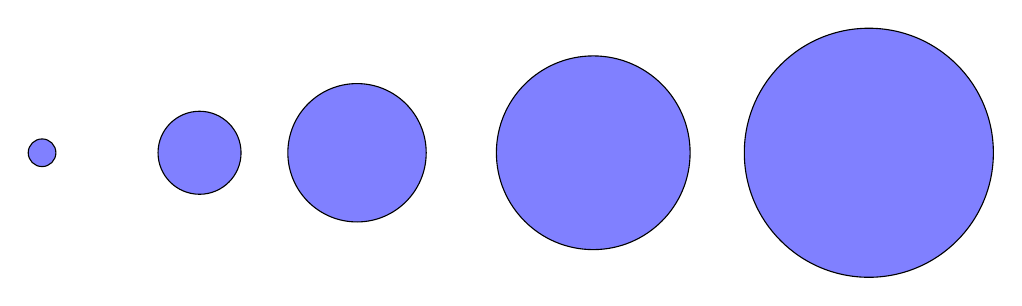
\begin{tikzpicture}
	\tikzstyle{un}=[circle,draw,fill=blue!50,minimum size=10pt]
	\tikzstyle{deux}=[circle,draw,fill=blue!50,minimum size=30pt]
	\tikzstyle{trois}=[circle,draw,fill=blue!50,minimum size=50pt]
	\tikzstyle{quatre}=[circle,draw,fill=blue!50,minimum size=70pt]
	\tikzstyle{cinq}=[circle,draw,fill=blue!50,minimum size=90pt]
	\node[un] (A) at (0,0){ };
	\node[deux] (B) at (2,0){ };
	\node[trois] (C) at (4,0){ };
	\node[quatre] (D) at (7,0){ };
	\node[cinq] (E) at (10.5,0){};
\end{tikzpicture}
\end{center}

\begin{center}
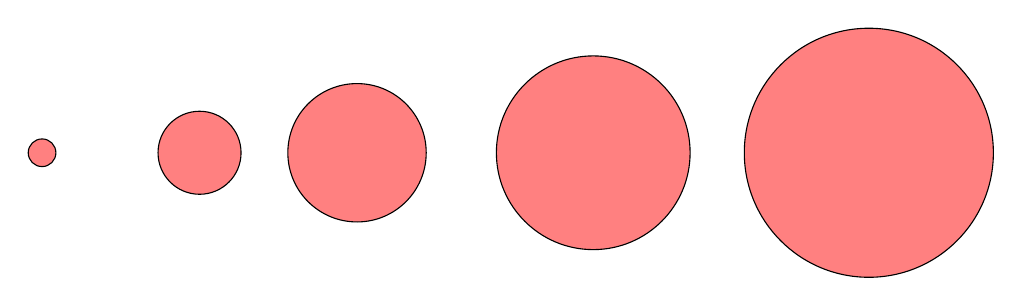
\begin{tikzpicture}
	\tikzstyle{un}=[circle,draw,fill=red!50,minimum size=10pt]
	\tikzstyle{deux}=[circle,draw,fill=red!50,minimum size=30pt]
	\tikzstyle{trois}=[circle,draw,fill=red!50,minimum size=50pt]
	\tikzstyle{quatre}=[circle,draw,fill=red!50,minimum size=70pt]
	\tikzstyle{cinq}=[circle,draw,fill=red!50,minimum size=90pt]
	\node[un] (A) at (0,0){ };
	\node[deux] (B) at (2,0){ };
	\node[trois] (C) at (4,0){ };
	\node[quatre] (D) at (7,0){ };
	\node[cinq] (E) at (10.5,0){};
\end{tikzpicture}
\end{center}

\begin{center}
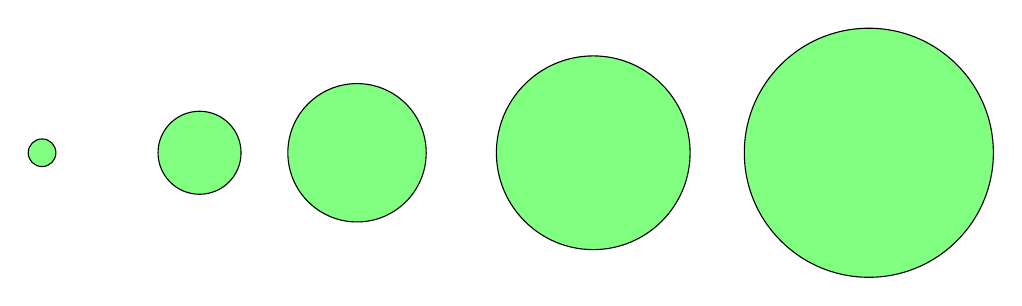
\begin{tikzpicture}
	\tikzstyle{un}=[circle,draw,fill=green!50,minimum size=10pt]
	\tikzstyle{deux}=[circle,draw,fill=green!50,minimum size=30pt]
	\tikzstyle{trois}=[circle,draw,fill=green!50,minimum size=50pt]
	\tikzstyle{quatre}=[circle,draw,fill=green!50,minimum size=70pt]
	\tikzstyle{cinq}=[circle,draw,fill=green!50,minimum size=90pt]
	\node[un] (A) at (0,0){ };
	\node[deux] (B) at (2,0){ };
	\node[trois] (C) at (4,0){ };
	\node[quatre] (D) at (7,0){ };
	\node[cinq] (E) at (10.5,0){};
\end{tikzpicture}
\end{center}

\begin{center}
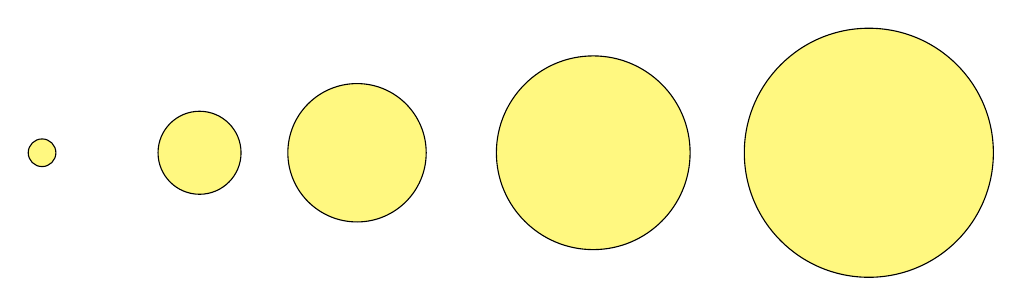
\begin{tikzpicture}
	\tikzstyle{un}=[circle,draw,fill=yellow!50,minimum size=10pt]
	\tikzstyle{deux}=[circle,draw,fill=yellow!50,minimum size=30pt]
	\tikzstyle{trois}=[circle,draw,fill=yellow!50,minimum size=50pt]
	\tikzstyle{quatre}=[circle,draw,fill=yellow!50,minimum size=70pt]
	\tikzstyle{cinq}=[circle,draw,fill=yellow!50,minimum size=90pt]
	\node[un] (A) at (0,0){ };
	\node[deux] (B) at (2,0){ };
	\node[trois] (C) at (4,0){ };
	\node[quatre] (D) at (7,0){ };
	\node[cinq] (E) at (10.5,0){};
\end{tikzpicture}
\end{center}

\begin{center}
\begin{tikzpicture}
	\tikzstyle{un}=[circle,draw,fill=white!50,minimum size=10pt]
	\tikzstyle{deux}=[circle,draw,fill=white!50,minimum size=30pt]
	\tikzstyle{trois}=[circle,draw,fill=white!50,minimum size=50pt]
	\tikzstyle{quatre}=[circle,draw,fill=white!50,minimum size=70pt]
	\tikzstyle{cinq}=[circle,draw,fill=white!50,minimum size=90pt]
	\node[un] (A) at (0,0){ };
	\node[deux] (B) at (2,0){ };
	\node[trois] (C) at (4,0){ };
	\node[quatre] (D) at (7,0){ };
	\node[cinq] (E) at (10.5,0){};
\end{tikzpicture}
\end{center}
 
\begin{center}
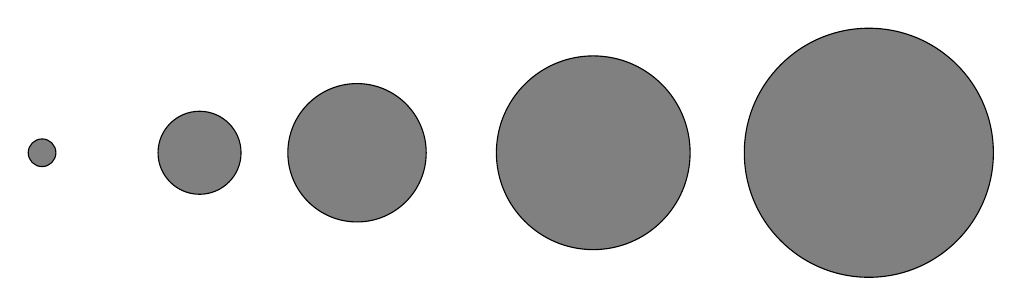
\begin{tikzpicture}
	\tikzstyle{un}=[circle,draw,fill=black!50,minimum size=10pt]
	\tikzstyle{deux}=[circle,draw,fill=black!50,minimum size=30pt]
	\tikzstyle{trois}=[circle,draw,fill=black!50,minimum size=50pt]
	\tikzstyle{quatre}=[circle,draw,fill=black!50,minimum size=70pt]
	\tikzstyle{cinq}=[circle,draw,fill=black!50,minimum size=90pt]
	\node[un] (A) at (0,0){ };
	\node[deux] (B) at (2,0){ };
	\node[trois] (C) at (4,0){ };
	\node[quatre] (D) at (7,0){ };
	\node[cinq] (E) at (10.5,0){};
\end{tikzpicture}
\end{center}

\newpage

\begin{center}
\begin{pgfpicture}
   \pgfmathdeclarerandomlist{color}{{red}{blue}{green}{yellow}{white}{black}}
   \foreach \a in {1,...,35}{
      \pgfmathrandominteger{\x}{1}{350}
      \pgfmathrandominteger{\y}{1}{600}
      \pgfmathrandominteger{\r}{4}{30}
      \pgfmathrandomitem{\c}{color}
      \pgfpathcircle{\pgfpoint{+\x pt}{+\y pt}}{+\r pt}
      \color{\c!50!white}
      \pgfsetstrokecolor{\c!90!black}
      \pgfusepath{stroke, fill}
   }
\end{pgfpicture}
\end{center}

%%%%%%%%%%%%%%%
%STRUCTURE BOUCLE%
%%%%%%%%%%%%%%
\chapter[Structure avec boucles : \greektext 
K'irkh e>upl'okamoc\latintext]{\greektext 
K'irkh e>upl'okamoc\latintext\textsuperscript{{\normalsize{\footnotemark}}}}
\chaptermark{\greektext K'irkh e>upl'okamoc\latintext}
\footnotetext{Circé aux belles boucles}

{\large \textbf{Catégorie}}:
structure avec boucles

%%\subsection*{Catégorie}
%{\large \textbf{Catégorie}}:
%communication

\section*{Cadre et public}
\begin{itemize}
\item [\textbullet]\textbf{Type d'atelier} : piano

\item [\textbullet]\textbf{Public} : 4 élèves (ou 3 élèves et le professeur) ayant terminé le cursus de formation musicale

\item [\textbullet]\textbf{Gestion du temps} : à répartir sur plusieurs cours

\item [\textbullet]\textbf{Matériel} : 1 piano (4 mains); un instrument à percussion à hauteur indéterminée (claves ou équivalent, par exemple)
\end{itemize}

\section*{Objectifs}
\begin{itemize}
\item respect d'une pulsation non exprimée
\item aborder une polyrythmie très courante en musique latino-américaine et de variété: \metric{4}{4} contre \metric{3+3+2}{8}
\end{itemize}

%\subsection*{Difficultés possibles}

\section*{Déroulement par étapes}
\begin{itemize}
\item travail séparé de chaque partie; pendant ce temps, les autres imaginent silencieusement leur partie
\item on n'ajoute une mesure que lorsque la précédente est stable et sûre
\end{itemize}

\subsection*{Prolongement}
Explication du lien avec l'Odyssée. On peut aussi, au contraire, partir de l'histoire de Circé pour en arriver à la partition

\includepdf[pages=-,fitpaper=true,pagecommand={}, scale=0.77]{boucles_euplokamos.pdf}

%\lilypondfile[indent=1\cm]{boucles_euplokamos.ly}

%%%%%%%%%%%%
%Consignes d'impro%
%%%%%%%%%%%%
\chapter{Trois consignes d'improvisations}

\section*{Consignes}
\begin{enumerate}
\item geste: \emph{arc-de-cercle dessiné du bras}
\item image: \emph{empreintes fossiles}
\item rôle: \emph{mélodie en mode lydien sur une basse I-V}
\end{enumerate}

\section*{Cadre et public}
\begin{itemize}
\item [\textbullet]\textbf{Type d'atelier} : tous

\item [\textbullet]\textbf{Public} : tous

\item [\textbullet]\textbf{Gestion du temps} : 5 minutes pour chaque, à répéter plusieurs fois sur l'année (avec d'autres consignes similaires)

%\item [\textbullet]\textbf{Matériel:} 
\end{itemize}

\section*{Objectifs}
\begin{itemize}
\item traduction musicale d'une consigne
\item écoute mutuelle
\item intégration du choix musical de chacun dans l'ensemble
\end{itemize}

%\subsection*{Difficultés possibles}

\section*{Déroulement par étapes}
\begin{itemize}
\item s'il y a beaucoup d'élèves, choisir un élève qui sera observateur
\item donner la consigne aux autres
\item laisser aux improvisateurs le soin de débuter et finir l'improvisation
\item faire deviner à l'observateur quelle était la consigne
\end{itemize}

%%%%%%%%%%%%%
%%Consignes d'impro%
%%%%%%%%%%%%%
%\chapter{Consigne d'improvisation 1 (gestes, images, rôles)}
%
%geste: arc-de-cercle dessiné du bras
%
%
%
%{\large \textbf{Sous-titre}}:
% consigne d'impro
%
%%%\subsection*{Catégorie}
%%{\large \textbf{Catégorie}}:
%%communication
%
%\section*{Cadre et public}
%\begin{itemize}
%\item [\textbullet]\textbf{Type d'atelier} : 
%
%\item [\textbullet]\textbf{Public} : 
%
%\item [\textbullet]\textbf{Gestion du temps:} 
%
%\item [\textbullet]\textbf{Matériel:} 
%\end{itemize}
%
%\section*{Objectifs}
%(Soyez le plus précis possible)
%\begin{itemize}
%\item test
%\item test
%\end{itemize}
%
%\subsection*{Difficultés possibles}
%
%\section*{Déroulement par étapes}
%(Echauffement, apprentissage, créativité)
%\begin{itemize}
%\item test
%\item test
%\end{itemize}
%
%%%%%%%%%%%%%
%%Consignes d'impro 2%
%%%%%%%%%%%%%
%\chapter{Consigne d'improvisation 2 (gestes, images rôles)}
%
%image: empreintes fossiles
%
%{\large \textbf{Sous-titre}}:
% consigne d'impro
%
%%%\subsection*{Catégorie}
%%{\large \textbf{Catégorie}}:
%%communication
%
%\section*{Cadre et public}
%\begin{itemize}
%\item [\textbullet]\textbf{Type d'atelier} : 
%
%\item [\textbullet]\textbf{Public} : 
%
%\item [\textbullet]\textbf{Gestion du temps:} 
%
%\item [\textbullet]\textbf{Matériel:} 
%\end{itemize}
%
%\section*{Objectifs}
%(Soyez le plus précis possible)
%\begin{itemize}
%\item test
%\item test
%\end{itemize}
%
%\subsection*{Difficultés possibles}
%
%\section*{Déroulement par étapes}
%(Echauffement, apprentissage, créativité)
%\begin{itemize}
%\item test
%\item test
%\end{itemize}
%
%%%%%%%%%%%%%
%%Consignes d'impro 3%
%%%%%%%%%%%%%
%\chapter{Consigne d'improvisation 3 (gestes, images rôles)}
%
%rôle: 
%
%
%{\large \textbf{Sous-titre}}:
% consigne d'impro
%
%%%\subsection*{Catégorie}
%%{\large \textbf{Catégorie}}:
%%communication
%
%\section*{Cadre et public}
%\begin{itemize}
%\item [\textbullet]\textbf{Type d'atelier} : 
%
%\item [\textbullet]\textbf{Public} : 
%
%\item [\textbullet]\textbf{Gestion du temps:} 
%
%\item [\textbullet]\textbf{Matériel:} 
%\end{itemize}
%
%\section*{Objectifs}
%(Soyez le plus précis possible)
%\begin{itemize}
%\item test
%\item test
%\end{itemize}
%
%\subsection*{Difficultés possibles}
%
%\section*{Déroulement par étapes}
%(Echauffement, apprentissage, créativité)
%\begin{itemize}
%\item test
%\item test
%\end{itemize}

%%%%%%%%%%%%%%%
%TEXTE + CHARPENTE%
%%%%%%%%%%%%%%
\chapter[Texte et charpente: Les montres molles]{Les montres molles}
\chaptermark{Les montres molles}

{\large \textbf{Catégorie}}:
 texte et charpente

%%\subsection*{Catégorie}
%{\large \textbf{Catégorie}}:
%communication

\section*{Cadre et public}
\begin{itemize}
\item [\textbullet]\textbf{Type d'atelier} : activité musicale en 1\iere{} et 2\ieme{} primaire

\item [\textbullet]\textbf{Public} : enfants de 6 à 8 ans

\item [\textbullet]\textbf{Gestion du temps:} : à répartir sur plusieurs cours

\item [\textbullet]\textbf{Matériel} : piano, instruments à percussion
\end{itemize}

\section*{Objectifs}
\begin{itemize}
\item association entre un élément du texte et un paramètre musical
\item traduction sonore de cette association 
\end{itemize}

\subsection*{Difficultés possibles}
Pour les élèves non francophones, les autres élèves peuvent expliquer certains termes ou expressions (\emph{mettre en boule}, par exemple) avec leurs propres mots.

\section*{Déroulement par étapes}
\begin{itemize}
\item si besoin, rappel des paramètres sonores avec lesquels on peut jouer (rythme, tessiture, etc.)
\item déterminer le rapport texte - paramètre musical
\end{itemize}

\section*{Prolongement}
Découverte du tableau \emph{La persistance de la mémoire} de Dali, ainsi qu'un passage de Fantasia 2000 (Disney) qui évoque l'idée (non réalisée) d'un épisode basé sur les montres molles.

\newpage	

\begin{quotation}\emph{Monsieur Monsieur se promène.\\}

\emph{Sur son chemin, il trouve des montres molles.\\}

\emph{Aussitôt, Monsieur Monsieur devient tout mou.\\}

\emph{Il s'étale comme une flaque.\\}

\emph{Ça le met en boule.\\}

\emph{Il pense à un cube, et il prend la forme d'un cube.\\}

\emph{Il pense à une pyramide. Et il prend la forme d'une pyramide.\\}

\emph{Il essaie de penser à lui-même, mais il pense à un champignon.\\}

\emph{Ou à un éléphant.\\}

\emph{Ou à un chapeau à secrets.\\}

\emph{Ça le fait penser à Mademoiselle Moiselle. Et soudain, il redevient lui-même.\\}

\og{} C'est tout moi! Tout entier, tout partout, je suis moi! \fg{} \emph{dit Monsieur Monsieur.}\footnote{Claude \textsc{Ponti}, \emph{Les montres molles}, Paris: L'école des loisirs, 2008}\end{quotation}

\includepdf[pages=-,fitpaper=true,pagecommand={}, scale=0.77]{montres_molles.pdf}


%%%%%%%%%%%%%%%
%PEINTURE + CHARPENTE%
%%%%%%%%%%%%%%
\chapter[Peinture et charpente: La grande vague de Kanagawa]{La grande vague de Kanagawa}
\chaptermark{La grande vague de Kanagawa}

{\large \textbf{Catégorie}}:
 peinture et charpente
 
\begin{figure}[ht!]
\begin{center}
\includegraphics[width=15cm]{hokusai.jpg}
\end{center}
\caption{{\textsc{Hokusai}, \emph{La grande vague de Kanagawa}}}
\end{figure}


%%\subsection*{Catégorie}
%{\large \textbf{Catégorie}}:
%communication

\section*{Cadre et public}
\begin{itemize}
\item [\textbullet]\textbf{Type d'atelier} : ensemble instrumental

\item [\textbullet]\textbf{Public} : tous

\item [\textbullet]\textbf{Gestion du temps} : 50 minutes

%\item [\textbullet]\textbf{Matériel:} 
\end{itemize}

\section*{Objectifs}
\begin{itemize}
\item travail sur les nuances: progression et extrêmes 
\item mise en place de signes pour changer de nuances en même temps
\end{itemize}

\subsection*{Difficultés possibles}
Pour les instruments sur lesquels les nuances indiquées ne sont pas possibles à toutes les tessitures, rechercher la tessiture la plus appropriée à la nuance demandée

\section*{Déroulement par étapes}
\begin{itemize}
\item choix d'un mode ou réservoir de notes à utiliser (pentatonique par exemple)
\item désignation d'un meneur qui indiquera les changements de nuances
\end{itemize}

\subsection*{Prolongement}
Mise en valeur des nuances dans d'autres partitions, particulièrement avec les élèves qui ont tendance à \emph{oublier} les dynamiques au profit des notes et du rythme


\vspace{0.2cm}
\renewcommand{\betweenLilyPondSystem}[1]{\vspace{10mm}\linebreak}

\lilypondfile{charpente_peinture.ly}

\renewcommand{\betweenLilyPondSystem}[1]{\vspace{5mm}\linebreak}

%%%%%%%%%%%%%%%%%%%%
%EXERCICE TECH SS PARTITION 1%
%%%%%%%%%%%%%%%%%%%%
\chapter[Exercice technique sans partition: 3 contre 2]{3 contre 2}
\chaptermark{3 contre 2}

{\large \textbf{Catégorie}}:
 exercice technique sans partition

%%\subsection*{Catégorie}
%{\large \textbf{Catégorie}}:
%communication

\section*{Cadre et public}
\begin{itemize}
\item [\textbullet]\textbf{Type d'atelier} : piano

\item [\textbullet]\textbf{Public} : élèves de qualification 1

\item [\textbullet]\textbf{Gestion du temps} : 5 minutes

%\item [\textbullet]\textbf{Matériel:} 
\end{itemize}

\section*{Objectifs}
\begin{itemize}
\item préparer le travail de superposition binaire--ternaire
\end{itemize}

%\subsection*{Difficultés possibles}

\section*{Déroulement par étapes}
\begin{itemize}
\item l'exercice se déroule couvercle fermé
\item installation d'une pulsation frappée par un des élèves
\item sur chaque pulsation, un autre élève frappe 2 fois de même vitesse avec la main gauche
\item après quelques fois, il fait pareil en main droite en frappant 3 fois
\item alternance de plus en plus fréquente, jusqu'à changer sur chaque temps
\end{itemize}

\subsection*{Prolongement}
Intégration de cet exercice dans le cadre plus large d'un cours complet consacré à une partition présentant cette difficulté


%%%%%%%%%%%%%%%%%%%%
%EXERCICE TECH SS PARTITION 2%
%%%%%%%%%%%%%%%%%%%%
\chapter[Exercice technique sans partition: Bottes de sept lieues]{Bottes de sept lieues}
\chaptermark{Bottes de sept lieues}

{\large \textbf{Catégorie}}:
 exercice technique sans partition

%%\subsection*{Catégorie}
%{\large \textbf{Catégorie}}:
%communication

\section*{Cadre et public}
\begin{itemize}
\item [\textbullet]\textbf{Type d'atelier} : piano

\item [\textbullet]\textbf{Public} : élèves de formation 5

\item [\textbullet]\textbf{Gestion du temps} : 5 minutes, à répéter de temps en temps

%\item [\textbullet]\textbf{Matériel:} 
\end{itemize}

\section*{Objectifs}
\begin{itemize}
\item gérer de manière détendue des grands déplacements
\end{itemize}

%\subsection*{Difficultés possibles}

\section*{Déroulement par étapes}
\begin{itemize}
\item choisir une tonalité en fonction de la partition travaillée
\item jouer une note de cette tonalité avec le pouce de droite, puis une octave plus haut avec le petit doigt; agrandir petit à petit l'intervalle
\item faire pareil avec le pouce à la place du petit doigt (en remplaçant l'extension par un déplacement)
\end{itemize}

\subsection*{Prolongement}
Appliquer le même travail à deux mains, tant en mouvement parallèle que contraire


%%%%%%%%%%%%%%%%%%%%
%EXERCICE TECH SS PARTITION 3%
%%%%%%%%%%%%%%%%%%%%
\chapter[Exercice technique sans partition: Pédale]{Pédale}
\chaptermark{Pédale}

{\large \textbf{Catégorie}}:
 exercice technique sans partition

%%\subsection*{Catégorie}
%{\large \textbf{Catégorie}}:
%communication

\section*{Cadre et public}
\begin{itemize}
\item [\textbullet]\textbf{Type d'atelier} : piano

\item [\textbullet]\textbf{Public} : élèves de F3 ou F4

\item [\textbullet]\textbf{Gestion du temps} : 10 minutes

%\item [\textbullet]\textbf{Matériel:} 
\end{itemize}

\section*{Objectifs}
\begin{itemize}
\item changer rapidement et proprement la pédale
\end{itemize}

\subsection*{Difficultés possibles}
Les très petits élèves n'arrivent pas aux pédales

\section*{Déroulement par étapes}
\begin{itemize}
\item écouter un court morceau joué par un autre élève ou le professeur (dans le registre médium ou grave, si possible)
\item faire définir par l'élève les changements de pédale
\item l'élève change la pédale pendant que l'autre joue le morceau
\end{itemize}

%%%%%%%%%%%%%%%
%CHARPENTE BAROQUE%
%%%%%%%%%%%%%%%
\chapter[Charpente baroque: Rondeau]{Rondeau}
\chaptermark{Rondeau}


%\subsection*{Sous-titre}
{\large \textbf{Catégorie}}: charpente baroque


%%\subsection*{Catégorie}
%{\large \textbf{Catégorie}}: Charpente baroque

\section*{Cadre et public}
\begin{itemize}
\item [\textbullet]\textbf{Type d'atelier} : cours de piano
\item [\textbullet]\textbf{Public} : 3 élèves ayant terminé leur cycle de formation musicale et minimum 3 années de cours à l'instrument
\item [\textbullet]\textbf{Gestion du temps} : à répartir sur plusieurs cours
%\item [\textbullet]\textbf{Matériel:} 
\end{itemize}

%\subsection*{Horaire et gestion du temps}

\subsection*{Répertoire}
Refrain du \emph{Rondeau} extrait de \emph{Abdelazer or The Moor's Revenge} (Purcell)

\lilypondfile{Rondeau_basse.ly}

%\subsection*{Besoins}


\section*{Objectifs}
\begin{itemize}
\item perception d'une structure répétée de 8 mesures (très fréquente en musique baroque, classique ou jazz)
\item écriture d'une mélodie sur cette ligne de basse
\end{itemize}

\subsection*{Difficultés possibles}
Avec des élèves adultes, il n'y a pas assez d'espace pour placer confortablement 3 personnes devant le piano; il faudra donc un deuxième clavier

\section*{Déroulement par étapes}
\begin{itemize}
\item travail collectif de la ligne de basse
\item travail collectif des accords sous forme d'arpèges; ils serviront ensuite d'accompagnement
\item création d'une mélodie en utilisant les notes des accords
\item enrichissement de la mélodie avec des notes de passage de et la figuration
\end{itemize}



%\subsection*{Feed-back possible}
%
%(Ce que vous pourriez dire aux participants)

\section*{Prolongements éventuels}
Le rondeau étant une alternance d'un refrain et de couplets, composition d'une partie B, en considérant la partie A comme refrain. Une fois ce travail fini, on peut faire écouter d'autres versions que celle proposée par les élèves : Purcell, mais également Britten.


%%%%%%%%%%%%%%%%%
%PROPO MUSICO-THEATRALE%
%%%%%%%%%%%%%%%%%
\chapter[Proposition musico-théâtrale: Fancy Free]{Fancy Free (Bernstein)}
\chaptermark{Fancy Free (Bernstein)}

{\large \textbf{Catégorie}}: proposition musico-théâtrale 

%%\subsection*{Catégorie}
%{\large \textbf{Catégorie}}: Proposition musico-théâtrale

\section*{Cadre et public}
\begin{itemize}
\item [\textbullet]\textbf{Type d'atelier} : cours d'ensemble instrumental
\item [\textbullet]\textbf{Public} : élèves ayant déjà déchiffré la partition
\item [\textbullet]\textbf{Gestion du temps} : à répartir sur plusieurs cours
\item [\textbullet]\textbf{Matériel} : l'effectif instrumental prévu dans l'arrangement (adapté à l'effectif de la classe); en cas de besoin, modification possible de l'arrangement
\end{itemize}

%\subsection*{Horaire et gestion du temps}


\subsection*{Répertoire}
\emph{Danzón}, extrait du ballet \emph{Fancy Free} (Bernstein)


\section*{Objectifs}
\begin{itemize}
\item aider les élèves à rendre le caractère de la partition
\item susciter la recherche par les élèves de leurs propres images et histoires
\end{itemize}

%\subsection*{Difficultés possibles}

\section*{Déroulement par étapes}
\begin{itemize}
\item jouer la partition sans prêter attention aux nuances ou intentions musicales
\item dégager les endroits particulier à mettre en évidence musicalement
\item raconter l'histoire servant de fil rouge aux didascalies et proposer des indications
\item propositions complémentaires ou contradictoires des élèves; fixation du choix des indications
\item exécution de la nouvelle version, et comparaison des deux exécutions
\end{itemize}


%
%\subsection*{Feed-back possible}
%
%(Ce que vous pourriez dire aux participants)

\section*{Prolongements éventuels}
\begin{itemize}
\item la récurrence de ce genre d'exercice amènera les élèves à appliquer cette recherche dans d'autres partitions et d'autres cours. 
\item à plus long terme, ce travail peut faire l'objet d'une collaboration avec le cours de danse 
\end{itemize}

\includepdf[pages=-,fitpaper=true,pagecommand={}, scale=0.77]{Bernstein-Danzon/Danzon.pdf}

%%%%%%%%%%
%COMPO PERSO%
%%%%%%%%%%
\chapter[Composition personnelle: Théorie des cordes]{Théorie des cordes}
\chaptermark{Théorie des cordes}
%Spacialisation ?
%
%Cordes (-> piano à queue, gommettes etc)
%
%{\large \textbf{Sous-titre}}:
% ?????????

%\subsection*{Catégorie}
{\large \textbf{Catégorie}}:
composition personnelle

\section*{Cadre et public}
\begin{itemize}
\item [\textbullet]\textbf{Type d'atelier} : piano

\item [\textbullet]\textbf{Public} : débutants

\item [\textbullet]\textbf{Gestion du temps} : à répartir sur plusieurs cours

\item [\textbullet]\textbf{Matériel} : en plus du piano, une paire de baguettes (marimba, vibraphone) ou, à défaut, de claves
\end{itemize}

\section*{Objectifs}
\begin{itemize}
\item habituer les élèves à des utilisations alternatives de l'instrument (cluster, cordes etc.)
\item installer un climat positif de jeu "sans erreur" par l'utilisation des seules touches blanches du piano (ici le mode dorien)
\item rechercher des alternatives au jeu dans les cordes si impossible (piano électrique, piano droit)
\end{itemize}

\subsection*{Difficultés possibles}
Absence d'un piano à queue. Dans ce cas, l'utilisation des cordes peut être remplacée par des clusters (piano électrique) ou un combinaison de clusters et de jeu dans les cordes (en ouvrant le bas du piano droit). Il est également possible d'avoir accès à un gong, un tam-tam voire une cymbale après de la classe de percussion. De plus, le jeu dans les cordes est plus difficiles avec les élèves de petite taille.

\section*{Déroulement par étapes}
\begin{itemize}
\item répartition des rôles (grave, aigu, cordes)
\item travail, par tous, de chaque partie
\item exécution complète, en s'assurant que chaque cellule est maîtrisée avant de passer à la suivante
\end{itemize}

\subsection*{Prolongement}
Travail d'autres partitions écrites en mode dorien (p. ex. Greensleeves)

\includepdf[pages=-,fitpaper=true,pagecommand={}, scale=0.77]{theorie_des_cordes.pdf}

%%%%%%%%%%%%%
%2 COURS COMPLET 2%
%%%%%%%%%%%%%
\chapter[Cours complet: 4 contre 3]{4 contre 3}
\chaptermark{4 contre 3}

%{\large \textbf{Sous-titre}}:
% ?????????

%\subsection*{Catégorie}
{\large \textbf{Catégorie}}:
cours complet

\section*{Cadre et public}
\begin{itemize}
\item [\textbullet]\textbf{Type d'atelier} : cours de piano

\item [\textbullet]\textbf{Public} : élèves en fin de filière de transition ou qualification

\item [\textbullet]\textbf{Gestion du temps} : 50 minutes

%\item [\textbullet]\textbf{Matériel:} un piano
\end{itemize}

\section*{Objectifs}
\begin{itemize}
\item mise en place d'une combinaison 4 croches contre triolet de noires
\item maintien d'un jeu souple malgré le respect de la polyrythmie
\end{itemize}

\subsection*{Répertoire}
Chopin, \emph{Trois nouvelles études} \no{}1

%\includepdf[pages=-,fitpaper=true,pagecommand={}, scale=0.77]{chopin_nouvelles_etudes_1.pdf}
\begin{center}\includegraphics[width=13.2cm]{chopin_nouvelles_etudes_1.pdf}\end{center}

%\subsection*{Difficultés possibles}
%x

\section*{Déroulement par étapes}
\begin{itemize}
\item échauffement: en marchant sur place, faire des ronds avec les poignets
\item jeu musical: marcher dans la classe en comptant jusqu'à 3 sur chaque pas (triolet), puis jusqu'à 4 (4 croches); passer de l'un à l'autre de plus en plus fréquemment
\item installation d'une pulsation de blanche
\item création par les élèves d'un fragment mélodique sur 8 croches(en lien avec la tonalité du morceau); jouer des croches sur cette pulsation
\item faire pareil avec des triolets de noires
\item passer de l'un à l'autre, d'abord peu fréquemment, puis de plus en plus souvent
\item attribuer un des deux rythmes à chaque élève
\item réalisation du 4 contre 3 sur ces mêmes notes
\item passage à la partition, d'abord mains séparées puis ensemble
\end{itemize}

%%%%%%%%%%%%%
%2 COURS COMPLET 2%
%%%%%%%%%%%%%
\chapter[Cours complet: Les moutons de Panurge]{Les moutons de Panurge}
\chaptermark{Les moutons de Panurge}


%\subsection*{Catégorie}
{\large \textbf{Catégorie}}:
cours complet

\section*{Cadre et public}
\begin{itemize}
\item [\textbullet]\textbf{Type d'atelier} : cours d'instrument ou d'ensemble instrumental

\item [\textbullet]\textbf{Public} : élèves de 5 années d'expérience minimum à l'instrument

\item [\textbullet]\textbf{Gestion du temps} : 50 minutes

%\item [\textbullet]\textbf{Matériel:} 
\end{itemize}

\subsection*{Répertoire}
Frederic Rzewski, \emph{Les moutons de Panurge}

\section*{Objectifs}
\begin{itemize}
\item déchiffrer une partition qui utilise des conventions de notations inhabituelles et nouvelles
\item maintenir une pulsation régulière, indispensable au jeu collectif
\item intégrer le risque d'erreur (ne pas se laisser influencer par les décalages probables)
\end{itemize}

\subsection*{Difficultés possibles}
Pour les instruments transpositeurs, prévoir une partition adaptée à leur tonalité

\section*{Déroulement par étapes}
\begin{itemize}
\item échauffement: débout, hausser les épaules en inspirant, puis relâcher brusquement les épaules en expirant; répéter 5 fois
\item jeu musical: tout le monde frappe; lorsqu'une même vitesse est atteinte, tout le monde compte jusqu'à 10 en même temps, en boucle. Un des élèves saute volontairement un chiffre, provoquant ainsi un décalage; continuer sans combler ce décalage
\item tâche de création: toujours à la même vitesse, un des participants donne le nom d'une note et le nom d'un autre élève. Le suivant reprend la même note, en ajoute une et donne le nom de l'élève suivant, et ainsi de suite.
\item départ depuis un extrait transcrit en notation traditionnelle; travail de lecture et vérification de la stabilité rythmique sur ce fragment, sans influence de la notation particulière
\item mise en parallèle de la version « retranscrite » et de la partition telle que le compositeur l’a écrite
\item discussion sur le titre (référence littéraire)
\item lecture et compréhension des instructions du compositeur
\item lecture de la partition par les élèves; en cas de difficulté plus importante chez l’un des  élèves, travail individuel avec soutien rythmique (pulsation) du ou des autres
\item jouer la partition ensemble, en respectant les notes, valeurs rythmiques et instructions particulières, y compris le risque d’erreur
\end{itemize}

\subsection*{Prolongement}
Réalisation par les élèves d’une partition basée sur un principe d’écriture similaire


%%%%%%%%%%%%%
%PROPO TRIMESTRE %
%%%%%%%%%%%%%
\chapter[Projet de trimestre: Le \emph{Musikalisches Würfelspiel} de Mozart]{Le \emph{Musikalisches Würfelspiel} de Mozart}
\chaptermark{Le \emph{Musikalisches Würfelspiel} de Mozart}


%\subsection*{Catégorie}
{\large \textbf{Catégorie}}:
projet de trimestre

\section*{Cadre et public}
\begin{itemize}
\item [\textbullet]\textbf{Type d'atelier} : collaboration entre les classes de piano, ensemble instrumental et formation musicale. L'accent est mis sur la synergie entre les différentes classes

\item [\textbullet]\textbf{Public} : élèves ayant suivi au moins 3 années de formation musicale

\item [\textbullet]\textbf{Gestion du temps} : à répartir sur un trimestre

\item [\textbullet]\textbf{Matériel} : 1 piano et l'instrument de chaque participant; un tableau aimanté pour placer les extraits de la partition dans l'ordre tiré au sort
\end{itemize}

\section*{Objectifs}
\begin{itemize}
\item composition d'une valse en suivant les indications de Mozart
\item déterminer collectivement une instrumentation
\item mettre en évidence les enchaînement harmoniques qui rendent possible ce genre de composition
\end{itemize}

\subsection*{Répertoire}
Mozart, \emph{Musikalisches Würfelspiel} sous forme de jeu de cartes, 2 dés et tableau des correspondances dés--mesure

\subsection*{Difficultés possibles}
Pour l'instrumentation, ne pas oublier les instruments transpositeurs. C'est l'occasion où jamais d'aborder la problématique de la transposition.

\section*{Déroulement par étapes}
\begin{itemize}
\item explication des règles du jeu
\item chacun à son tour lance les dés pour déterminer les mesures de la composition
\item les fragments tirés au sort sont placés sur un tableau 
\item répartition des rôles (accompagnement pour les instruments graves, mélodie pour les instruments aigus)
\item ré-écriture des différentes parties en fonction de l'instrumentation définie en classe (ce travail peut faire l'objet d'un travail en collaboration avec un cours de musique assistée par ordinateur)
\item mise en place et travail de la partition (sur plusieurs cours)
\item mise en évidence de la structure harmonique, pour répondre à la question "Pourquoi et comment ça marche?"
\item réalisation par les élèves d’une partition basée sur un principe d’écriture similaire
\end{itemize}

\section*{Finalités}
\begin{itemize}
\item exécution de la partition instrumentée lors du concert de fin d'année
\item exécution de plusieurs des partitions d'élèves réalisées suivant le même principe
\end{itemize}


\end{document}